%====================================================================================================
% ?????
%====================================================================================================
% TCC
%----------------------------------------------------------------------------------------------------
% Autor				: Jasane Schio
% Orientador		: Gedson Faria
% Co-Orientador		: Angelo Darcy
% Instituição 		: UFMS - Universidade Federal do Mato Grosso do Sul
% Departamento		: CPCX - Sistema de Informação
%----------------------------------------------------------------------------------------------------
% Data de criação	: 01 de Outubro de 2015
%====================================================================================================
% 
\chapter{Testes e Resultados} 
\section{Considerações Iniciais}
Este capítulo está divido em duas seções, nas quais estão presente os testes realizados bem como se discute os mesmos. Primeiramente se descreve o processo de calibração de cores bem como a preparação do campo, configuração de imagem, e seu resultado. Em seguida são apresentados os resultados dos testes executados com o arquivo gerado na calibração. Os resultados foram separados em Cores Comuns e Cores com Problemas. Por último se faz uma análise geral dos resultados obtidos.


 Para realização dos testes foi desenvolvido um aplicativo Desktop para fazer a leitura do arquivo gerado pela calibração, que possibilita a exibição de uma imagem contendo os objetos de acordo com a cor selecionada, por meio de um menu de escolha. Sendo assim possível a análise dos resultados obtidos para cada uma das cores. 
 
  O teste foi feito de uma só vez, porém sua análise está separada em duas partes. A primeira parte Cores Comuns, são as cores que não apresentam problema devido a semelhança com outras cores, na qual estava presente as cores amarelo, azul, verde, rosa, roxo. Na segunda parte estão presente as Cores com Problemas, que contém as cores vermelho e laranja. 
 
 A seguir está detalhado o processo de calibração, bem como a maneira com que o mesmo ocorreu. Após a explanação da calibração estão exposto os resultados deste teste e a validação de cada um.
\section{Calibração}
A calibração descrita a seguir ocorreu no dia 19 de Agosto de 2016, entre 17:36 e 17:39.
A rotina de calibração do sistema, já descrita no Capítulo 3, envolve primeiramente uma aquisição da imagem do campo vazio, como visto na Figura \ref{campovazio}.
\begin{figure}[H]
		\centering
		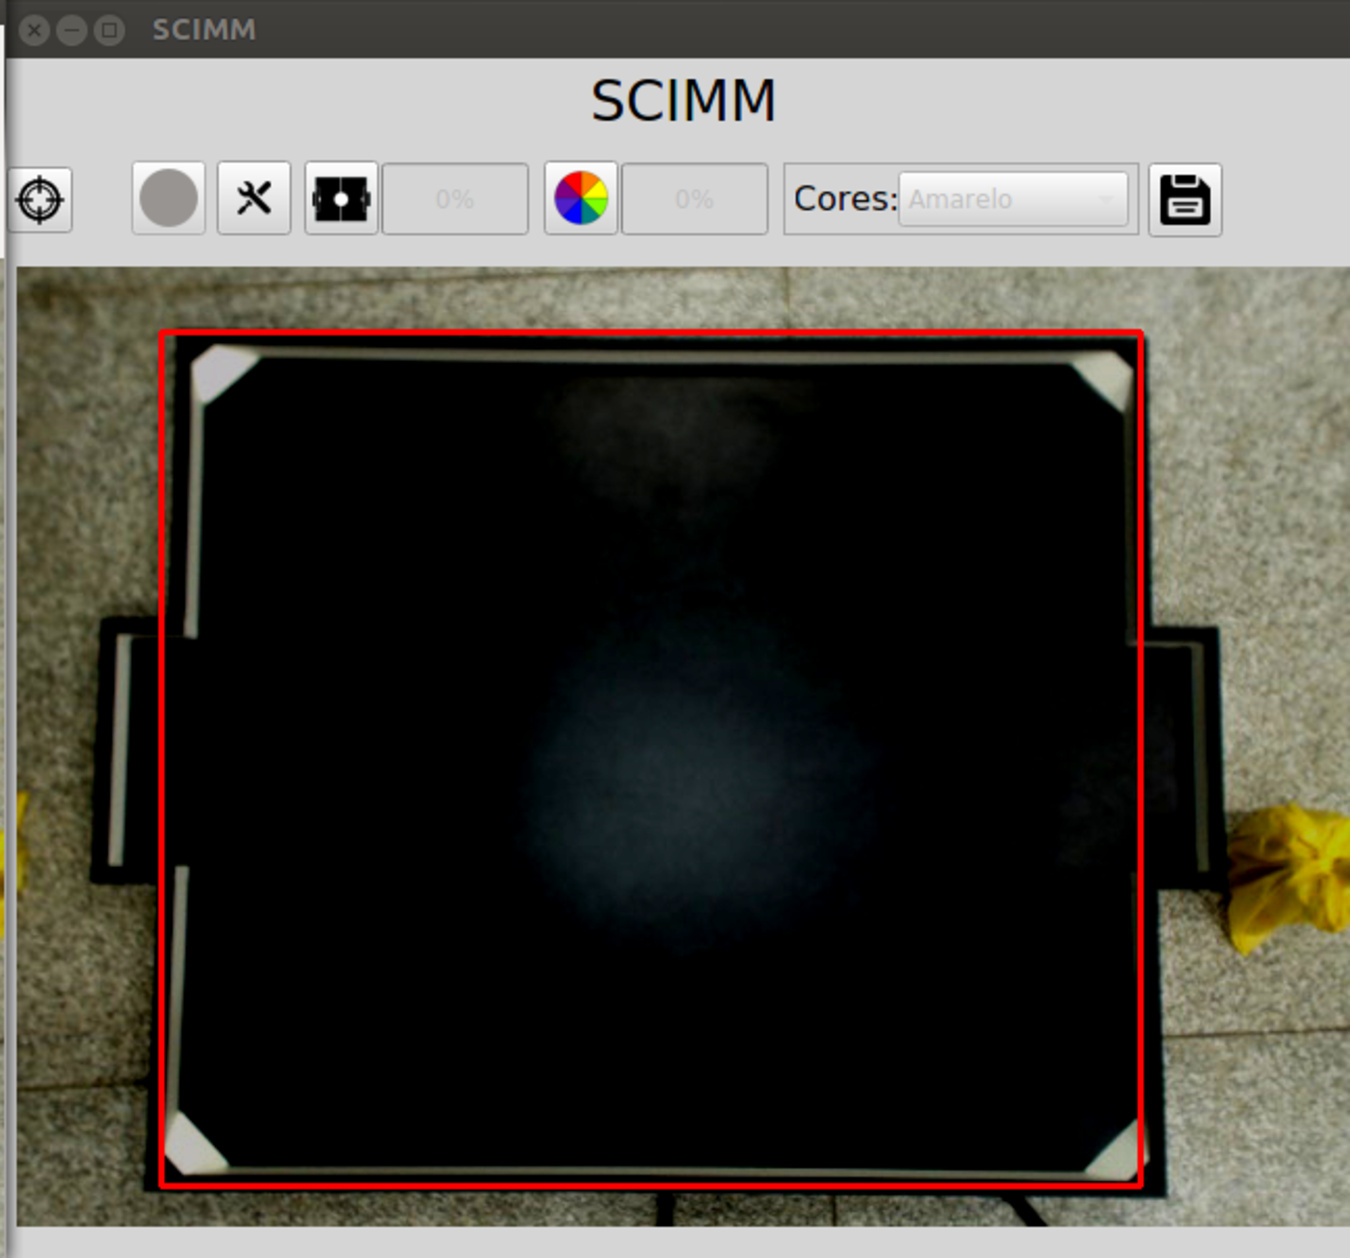
\includegraphics[width=0.45\textwidth]{fundoteste.pdf}
		\caption{Imagem do fundo com a seleção de campo}
		\label{campovazio}
	\end{figure}
	
Após ter o campo identificado pelo sistema, deve-se dispor sobre o campo os objetos coloridos, com as cores que se deseja obter o intervalo. É preferido que se usem tiras coloridas, pois quanto maior o tamanho da tira de cor, maior a quantidade de pixeis representando os vários espectros da cor, melhorando sensivelmente o processo de calibração.

Neste teste foram dispostos no campo tiras coloridas com largura entre \textit{17cm} e \textit{40cm} e altura entre \textit{5,5cm} e \textit{10,5cm}. Cada cor com 3 tiras, uma vez que o campo foi separado em três partes, com a finalidade de capturar diferentes luminosidades. A disposição das tiras pode ser vista na Figura \ref{fig:objetodispostos}.
	
	\begin{figure}[H]
%\begin{minipage}[H]{0.34\linewidth}
%\hspace{0.5cm}
\centering
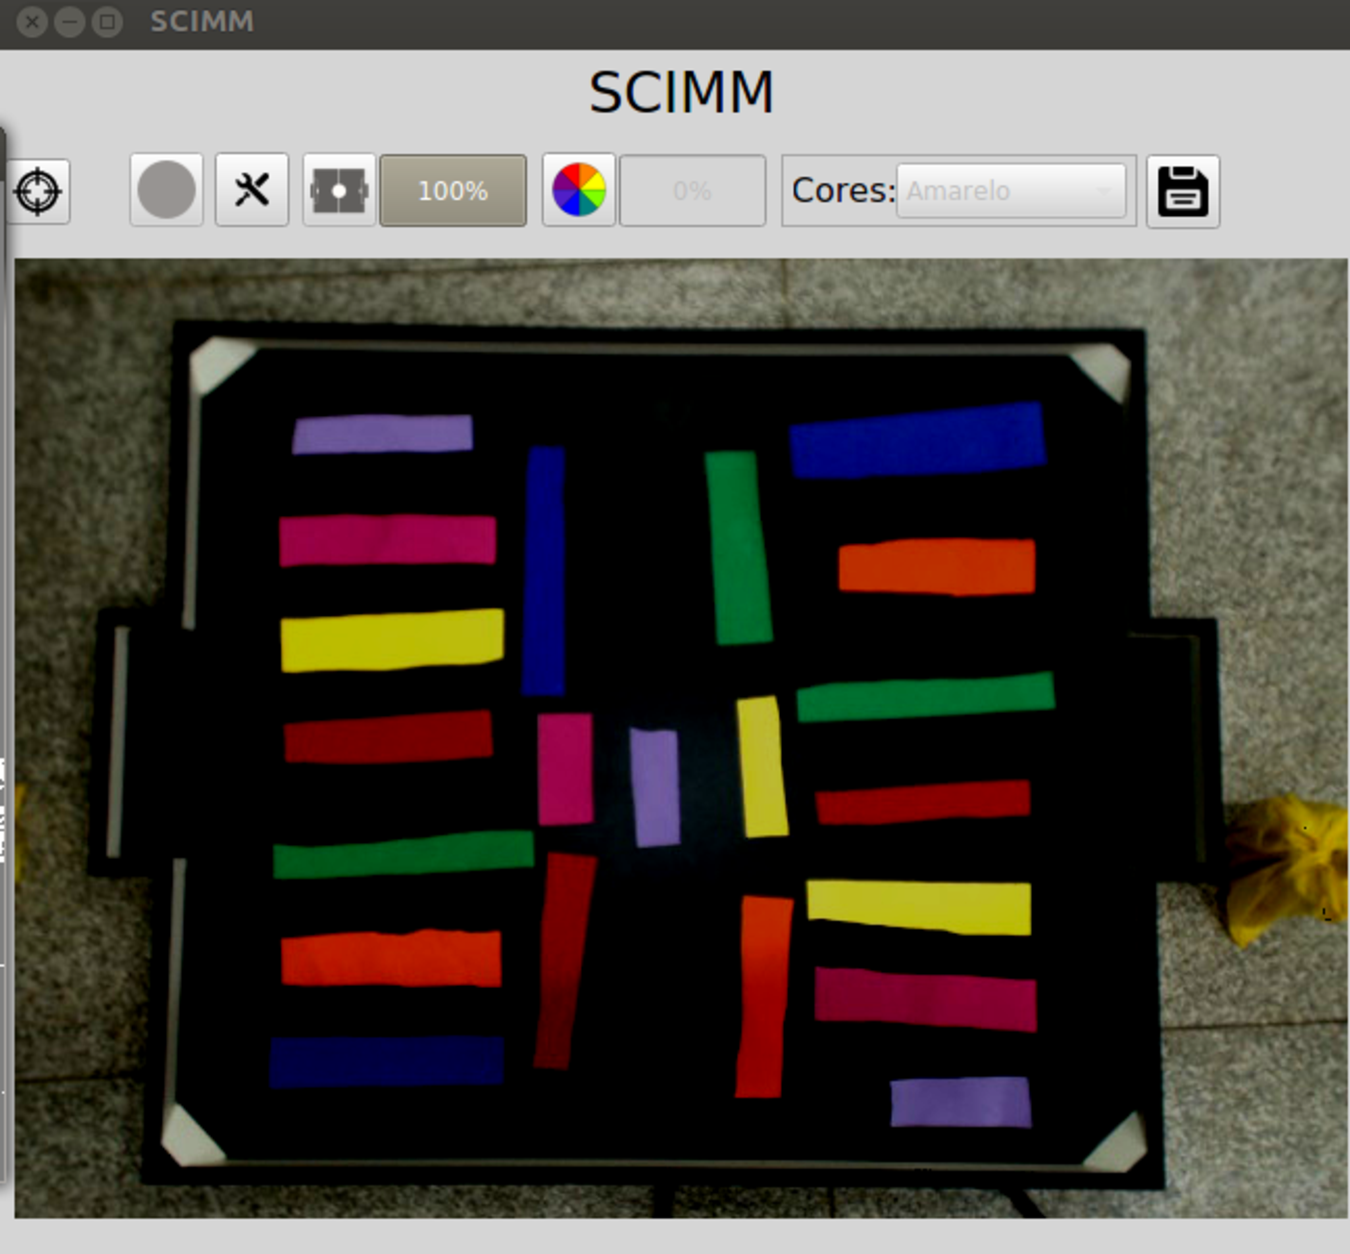
\includegraphics[width=0.45\textwidth]{objetosdispostos.pdf}
\caption{Objetos dispostos no campo para calibração}
\label{fig:objetodispostos}
%\end{minipage}
%\hspace{0.5cm}
%\begin{minipage}[H]{0.40\linewidth}
%\centering
%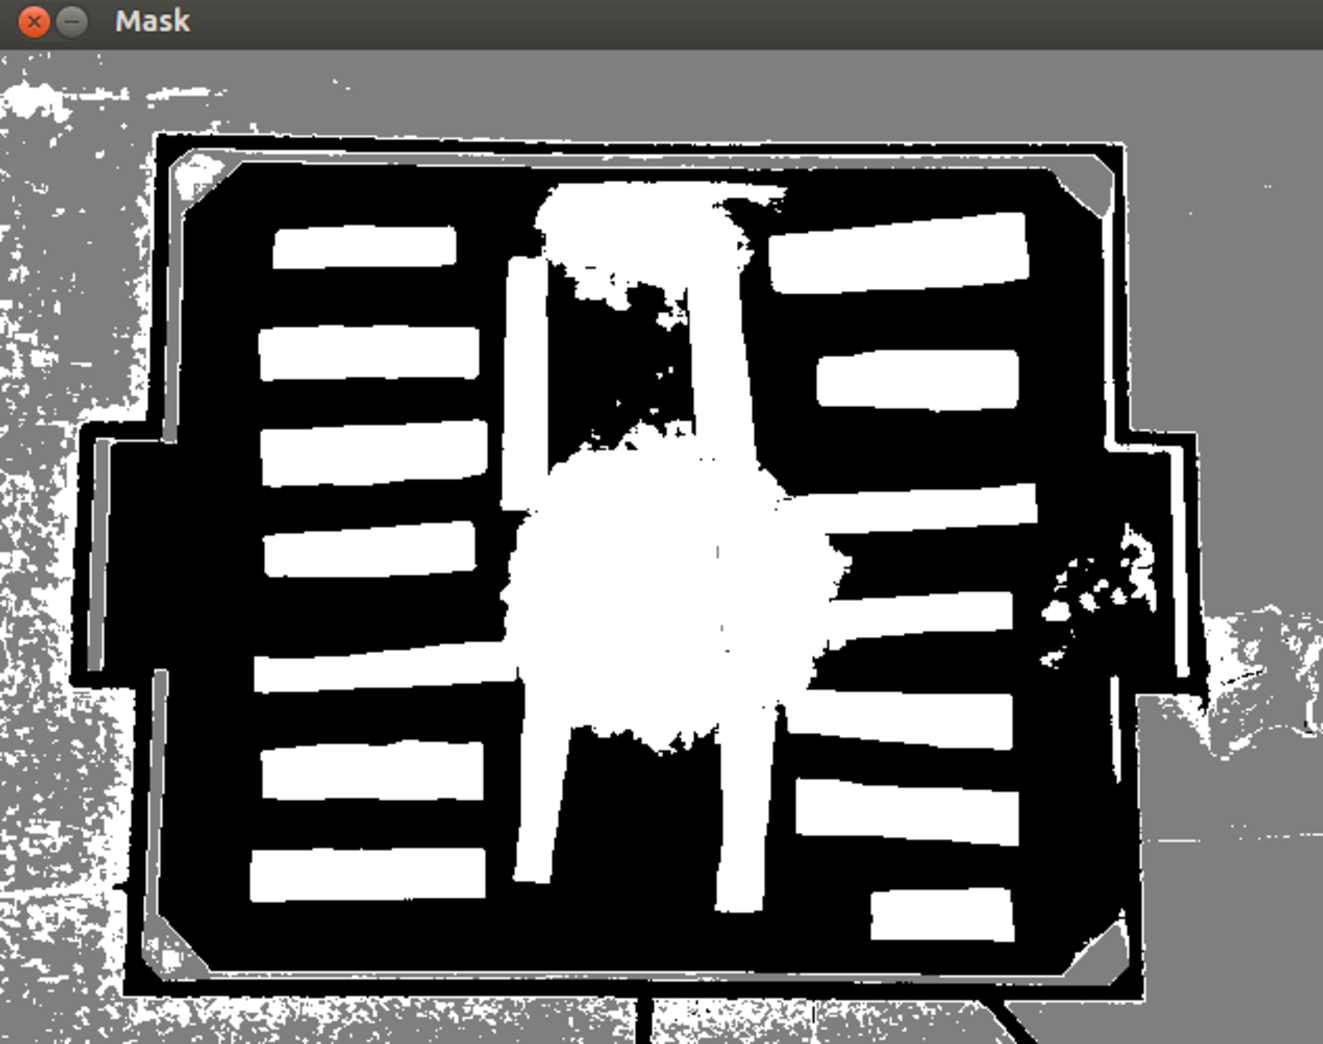
\includegraphics[width=\textwidth]{mascaragerada.pdf}
%\caption{Mascara gerada a partir da subtração de fundo}
%\label{fig:mascaragerada}
%\end{minipage}
\end{figure}	
	
Como resultado da rotina de calibração, foi gerado um arquivo .arff contendo 14 linhas. A Tabela \ref{tab:arquivo} possui uma explicação sobre o arquivo gerado. A primeira coluna da tabela designa a linha contida no arquivo, a segunda coluna possui o conteúdo existente no arquivo, na última coluna está a descrição do conteúdo de cada linha do arquivo.
	\begin{table}[H]
\centering 
\begin{tabular}{l|c|l}
Linha & Conteúdo & Descrição  \\% Note a separação de col. e a quebra de linhas
\hline                               % para uma linha horizontal
 1& 21.50.50  &   Valor mínimo da cor Amarelo \\ \hline  
2& 30.255.255  &  Valor máximo da cor Amarelo \\  \hline 
3& 92.100.100  &   Valor mínimo da cor Azul \\  \hline 
4& 120.255.255  &  Valor máximo da cor  Azul \\  \hline 
5& 62.30.100 &  Valor mínimo da cor Verde \\  \hline 
6& 90.255.255  &  Valor máximo da cor Verde \\  \hline 
7& 169.100.100  &  Valor mínimo da cor Vermelho \\  \hline 
8& 179.255.255  &  Valor máximo da cor Vermelho \\   \hline 
9& 0.100.100  &  Valor mínimo da cor Laranja \\  \hline 
10& 20.255.255 &  Valor máximo da cor  Laranja \\  \hline 
11& 161.100.100 &  Valor mínimo da cor Rosa \\  \hline 
12& 168.255.255 &   Valor máximo da cor Rosa \\  \hline 
13& 126.30.30 &  Valor mínimo da cor Roxo \\  \hline 
14& 160.255.255 &  Valor máximo da cor Roxo \\  \hline 

\end{tabular}
\caption{Os valores de HSV estão separados por pontuação, H.S.V}
\label{tab:arquivo}
\end{table}





 \section{Testes}
O teste aqui descrito ocorreu dia no 26 de Agosto de 2016, entre 13:28 e 16:28.
Para elaboração do teste optou-se por dividir o campo no maior número de partes possíveis, e ainda assim que essas partes coubessem todas as 7 cores calibradas. Essa divisão foi feita para simular as cores em todas as partes possíveis do campo. Sendo assim, o campo foi divido em 15 partes de \textit{29cm x 41cm}, nomeadas alfabeticamente de A a O, como mostrado na Figura \ref{fig:campodivisao}.	
	\begin{figure}[H]
		\begin{minipage}[b]{0.45\linewidth}
				\centering
				\includegraphics[width=\textwidth]{campodivisao.pdf}
				\caption{Divisão do campo em quinze partes nomeadas alfabeticamente.}
				\label{fig:campodivisao}
		
		\end{minipage}
		\hspace{0.5cm}
		\begin{minipage}[b]{0.45\linewidth}
			\centering
			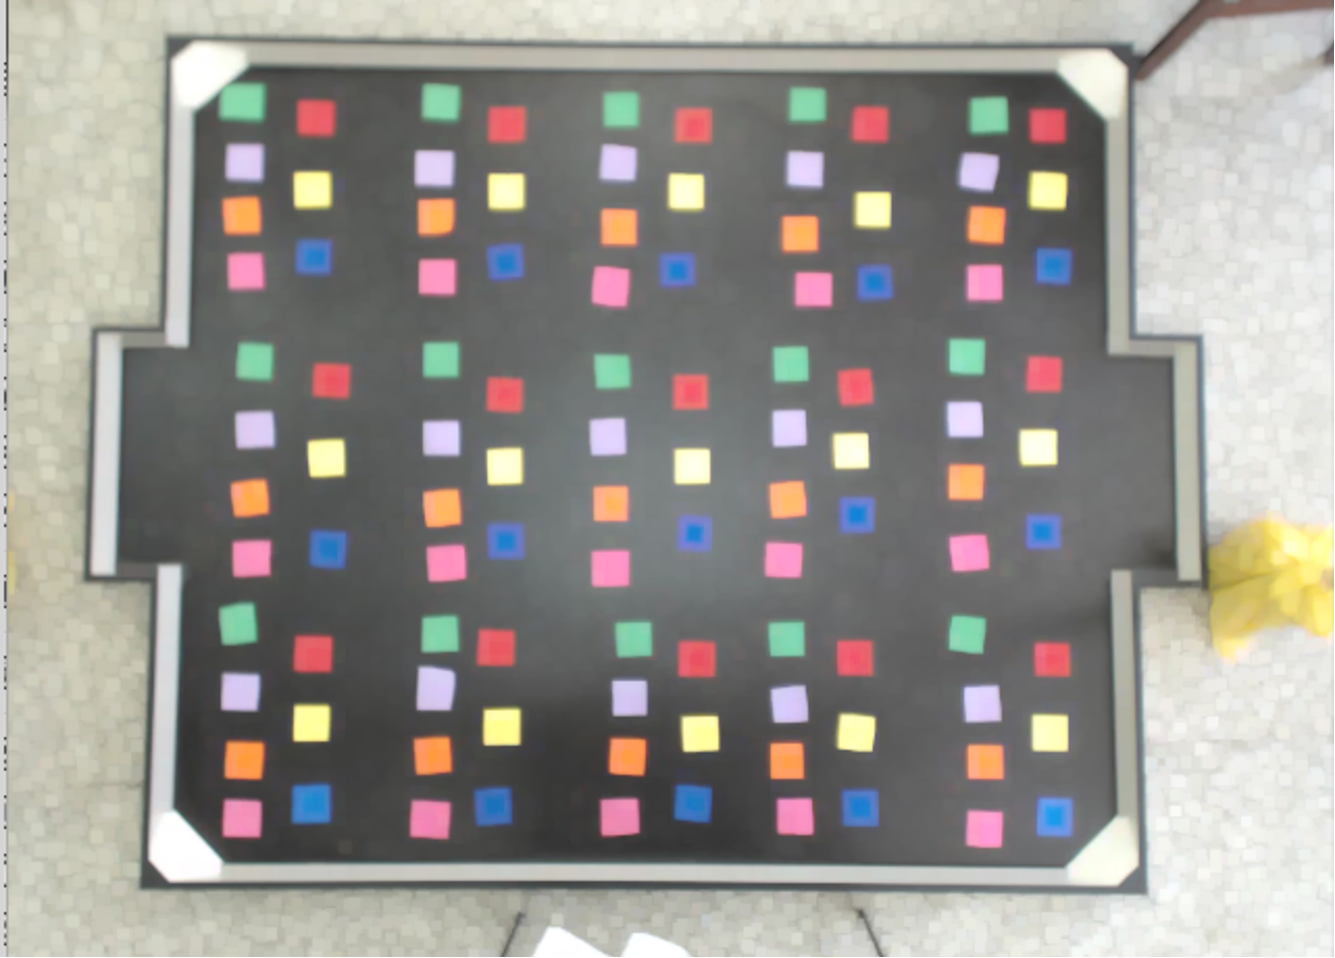
\includegraphics[width=\textwidth]{/testes/campofundo.pdf}
			\caption{Imagem do campo com marcadores de cores}
			\label{fig:figure2}
		\end{minipage}
	\end{figure}
	
Em cada uma das 15 partes do campo foi colocado marcadores representando as sete cores: Vermelho, Amarelo e Azul na primeira linha; Verde, Roxo, Laranja e Rosa na segunda. As cores estão distantes verticalmente \textit{6cm}. Na primeira linha a distância horizontal entre as cores é de \textit{7,25cm} e na segunda linha esta distância é de \textit{5cm}. Estas distâncias entre os marcadores de cores e suas disposições podem ser vistas nas Figuras \ref{fig:figure2} e \ref{fig:figure1}.

\begin{figure}[H]
	\centering
	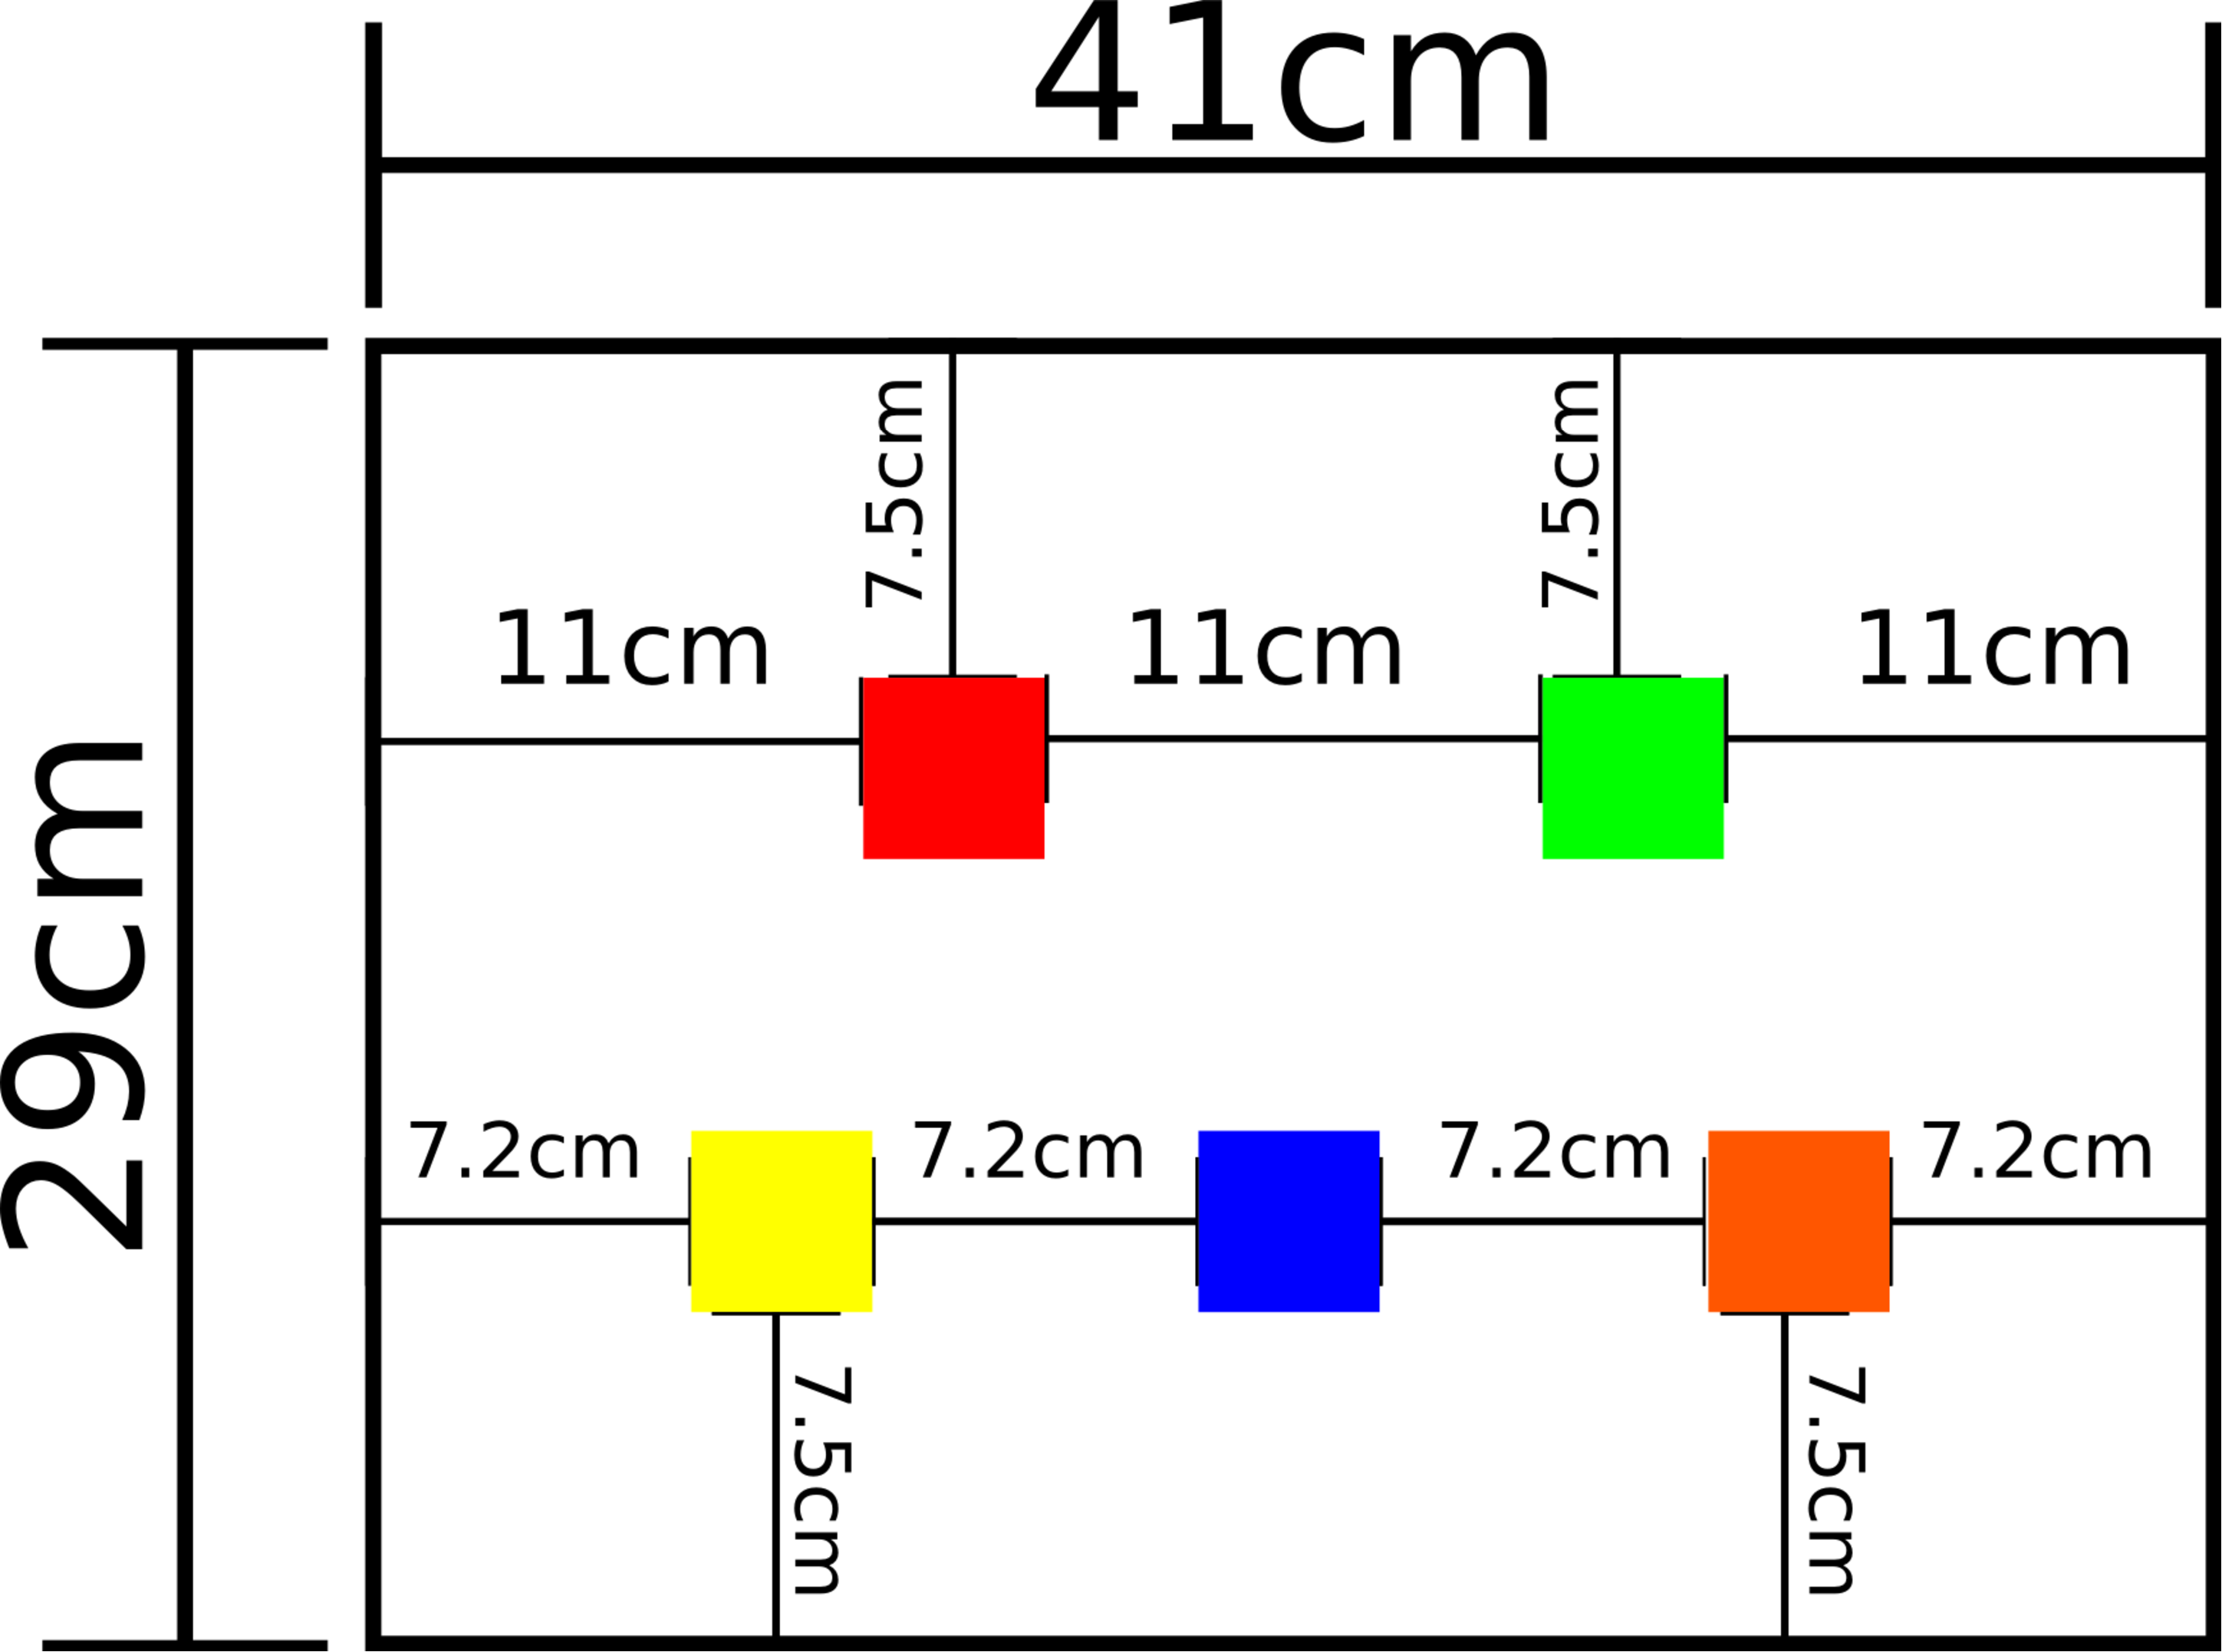
\includegraphics[width=.4\textwidth]{disposicaoparte.pdf}
	\caption{Disposição de cada parte quanto as cores}
	\label{fig:figure1}
\end{figure}

Quanto ao tipo de objeto encontrado, foram criados 7 categorias: Objetos Completos; Objetos com Falha de Preenchimento; Objetos com Diminuição de Contorno; Objetos com Diminuição de Área; Objetos com Falhas Críticas e Objetos Extrapolados.

\begin{description}
	\item[Objetos Completos] São os objetos que não contém nenhuma falha e foram encontrados corretamente.
		\item[Objetos com Falha de Preenchimento] São os objetos que contém apenas falha de preenchimento, contendo seu contorno encontrado de forma correta.
			\item[Objetos com Diminuição de Contorno] Foram os objetos encontrados com seu contorno reduzido devido á não detecção de sua borda.
				\item[Objetos com Diminuição de Área] Foram os objetos que foram encontrados porém sua área foi reduzida, e.g.Contém preenchimento e borda, mas a área encontrada é igual à metade do tamanho real do objeto.
					\item[Objetos com Falhas Críticas] São os objetos que apresentam mais de uma falha, diminuição de contorno, diminuição de borda ou diminuição de área. Estes objetos geralmente possuem sua aparência deformada, o que torna sua identificação pelos algoritmos de detecção de objetos
						\item[Objetos Extrapolados] São os objetos detectados dentro do intervalo uma cor especifica, que fazem parte de outra cor.
\end{description} 
\newpage
\subsection{Cores Comuns}
\subsubsection{Amarelo}	
	Dentre os objetos da cor amarela o sistema encontrou quatorze deles completamente (Figura \ref{fig:amarelo}), e apenas um, que devido a luminosidade implicada em seu centro deixando a tonalidade muito perto do branco, não totalmente preenchido. 
		\begin{figure}[H]
			\begin{minipage}[b]{0.45\linewidth}
				\centering
				\includegraphics[width=\textwidth]{campodivisao.pdf}
				\caption{Divisão do campo.}				
			\end{minipage}
			\hspace{0.5cm}
			\begin{minipage}[b]{0.45\linewidth}
				\centering
				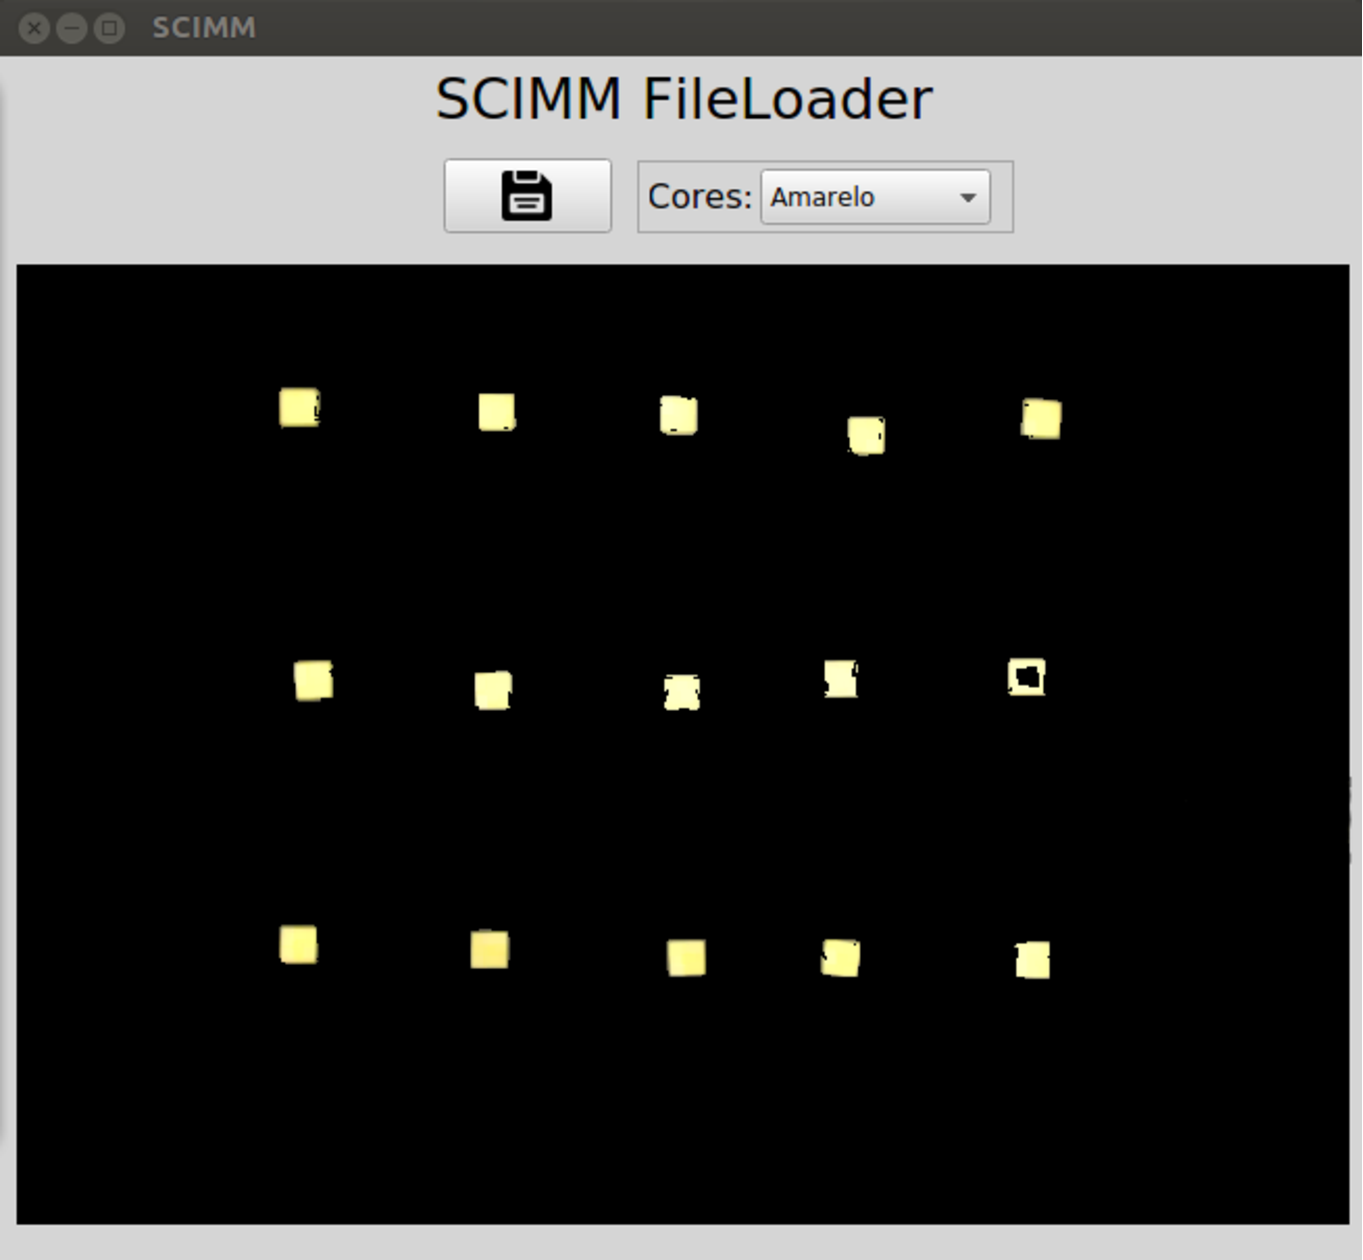
\includegraphics[width=\textwidth]{/testes/amarelo.pdf}
				\caption{Objetos da cor amarela}
				\label{fig:amarelo}
			\end{minipage}
		\end{figure}
	O único objeto detectado com falha encontra-se na parte N do campo.
	O detalhamento das quantidades e porcentagens dos objetos encontrados está na Tabela \ref{tab:amarelo}.
	
	\begin{table}[H]
\centering
\begin{tabular}{l|c|c}
Tipo de Objeto & Quantidade & \%  \\% Note a separação de col. e a quebra de linhas
\hline                               % para uma linha horizontal
Objetos Completos & 14 & 93,33 \\
\hline 
Objetos Com Falha de Preenchimento & 1 & 6,66 \\
\hline 
Objetos Com Diminuição de Contorno & 0 &\\
\hline 
Objetos Com Diminuição de Área &  0 &\\
\hline 
Objetos Com Falhas Críticas & 0 &\\
\hline \hline 
Objetos Extrapolados & 0 &\\
\hline 
\end{tabular}
\caption{Categorização Dos Objetos}
\label{tab:amarelo}
\end{table}

Dentre as classificações dos objetos as que descaracterizam o objeto para detecção são: \textit{Objetos Com Falhas Críticas} e \textit{Objetos Com Falha de Preenchimento}, que  para a cor amarelo resultou em 6,66\% dos objetos.

\newpage
\subsubsection{Azul}

Os objetos da cor azul foram os que obtiveram os melhores resultados, os quinze objetos foram encontrados de forma preenchida. Apesar dos quinze estarem totalmente preenchidos um dos objetos apresentou um tamanho reduzido aos demais devido ao fato de sua borda não ter sido totalmente detectada(Figura \ref{fig:azul}).
	\begin{figure}[H]
		\begin{minipage}[b]{0.45\linewidth}
			\centering
			\includegraphics[width=\textwidth]{campodivisao.pdf}
			\caption{Divisão do campo.}				
		\end{minipage}
		\hspace{0.5cm}
		\begin{minipage}[b]{0.45\linewidth}
			\centering
			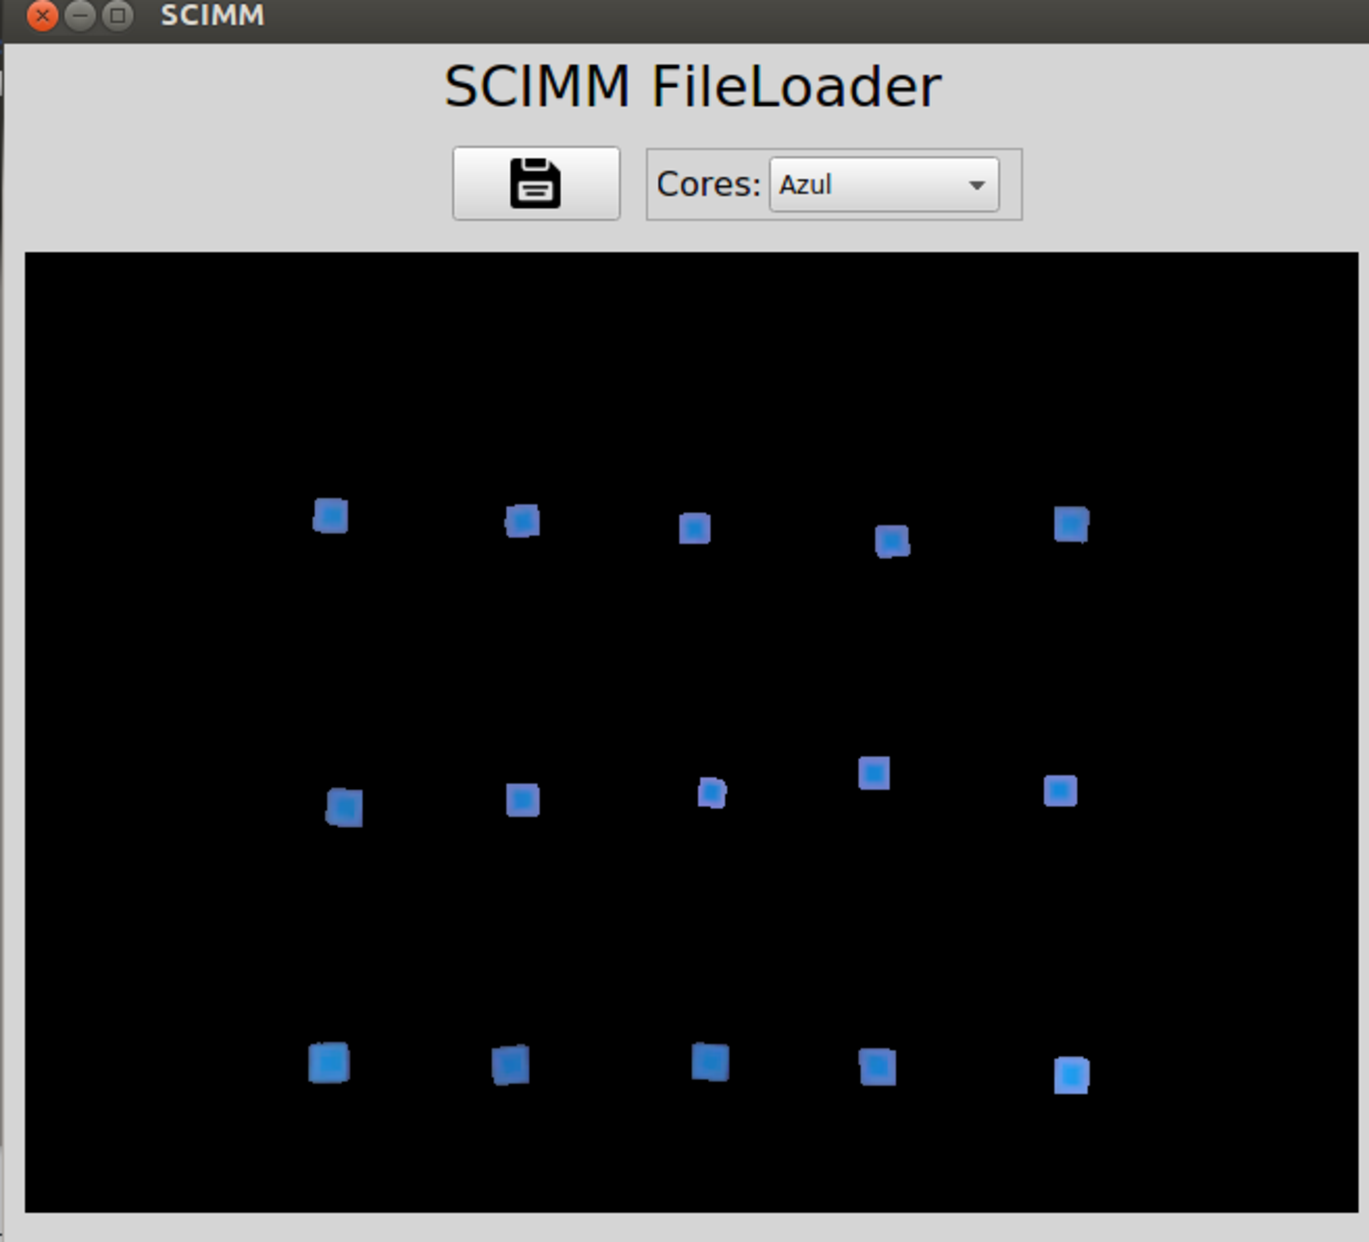
\includegraphics[width=\textwidth]{/testes/azul.pdf}
			\caption{Os objetos da cor azul}
			\label{fig:azul}
		\end{minipage}
	\end{figure}


O único objeto que conteve falha está presente na parte H do campo. Este não teve sua borda identificada dentro do intervalo de cor. O detalhamento das quantidades e porcentagens dos objetos encontrados está na Tabela \ref{tab:azul}.
\begin{table}[H]
\centering
\begin{tabular}{l|c|c}
Tipo de Objeto & Quantidade & \% \\ % Note a separação de col. e a quebra de linhas
\hline                               % para uma linha horizontal
Objetos Completos & 14 & 93,33 \\
\hline 
Objetos Com Falha de Preenchimento & 0\\
\hline 
Objetos Com Diminuição de Contorno &  1 & 6,66
\\
\hline 
Objetos Com Diminuição de Área & 0 \\
\hline 
Objetos Com Falhas Críticas & 0 \\
\hline \hline 
Objetos Extrapolados &  0\\
\hline 
\end{tabular}
\caption{Categorização Dos Objetos}
\label{tab:azul}
\end{table}
\newpage
\subsubsection{Verde}
Os objetos da cor verde foram satisfatoriamente encontrados, com seu preenchimento total e não havendo perda de área devido a qualquer interferência de luz em sua borda (Figura \ref{fig:verde}).	

	\begin{figure}[H]
		\begin{minipage}[b]{0.45\linewidth}
			\centering
			\includegraphics[width=\textwidth]{campodivisao.pdf}
			\caption{Divisão do campo.}				
		\end{minipage}
		\hspace{0.5cm}
		\begin{minipage}[b]{0.45\linewidth}
			\centering
			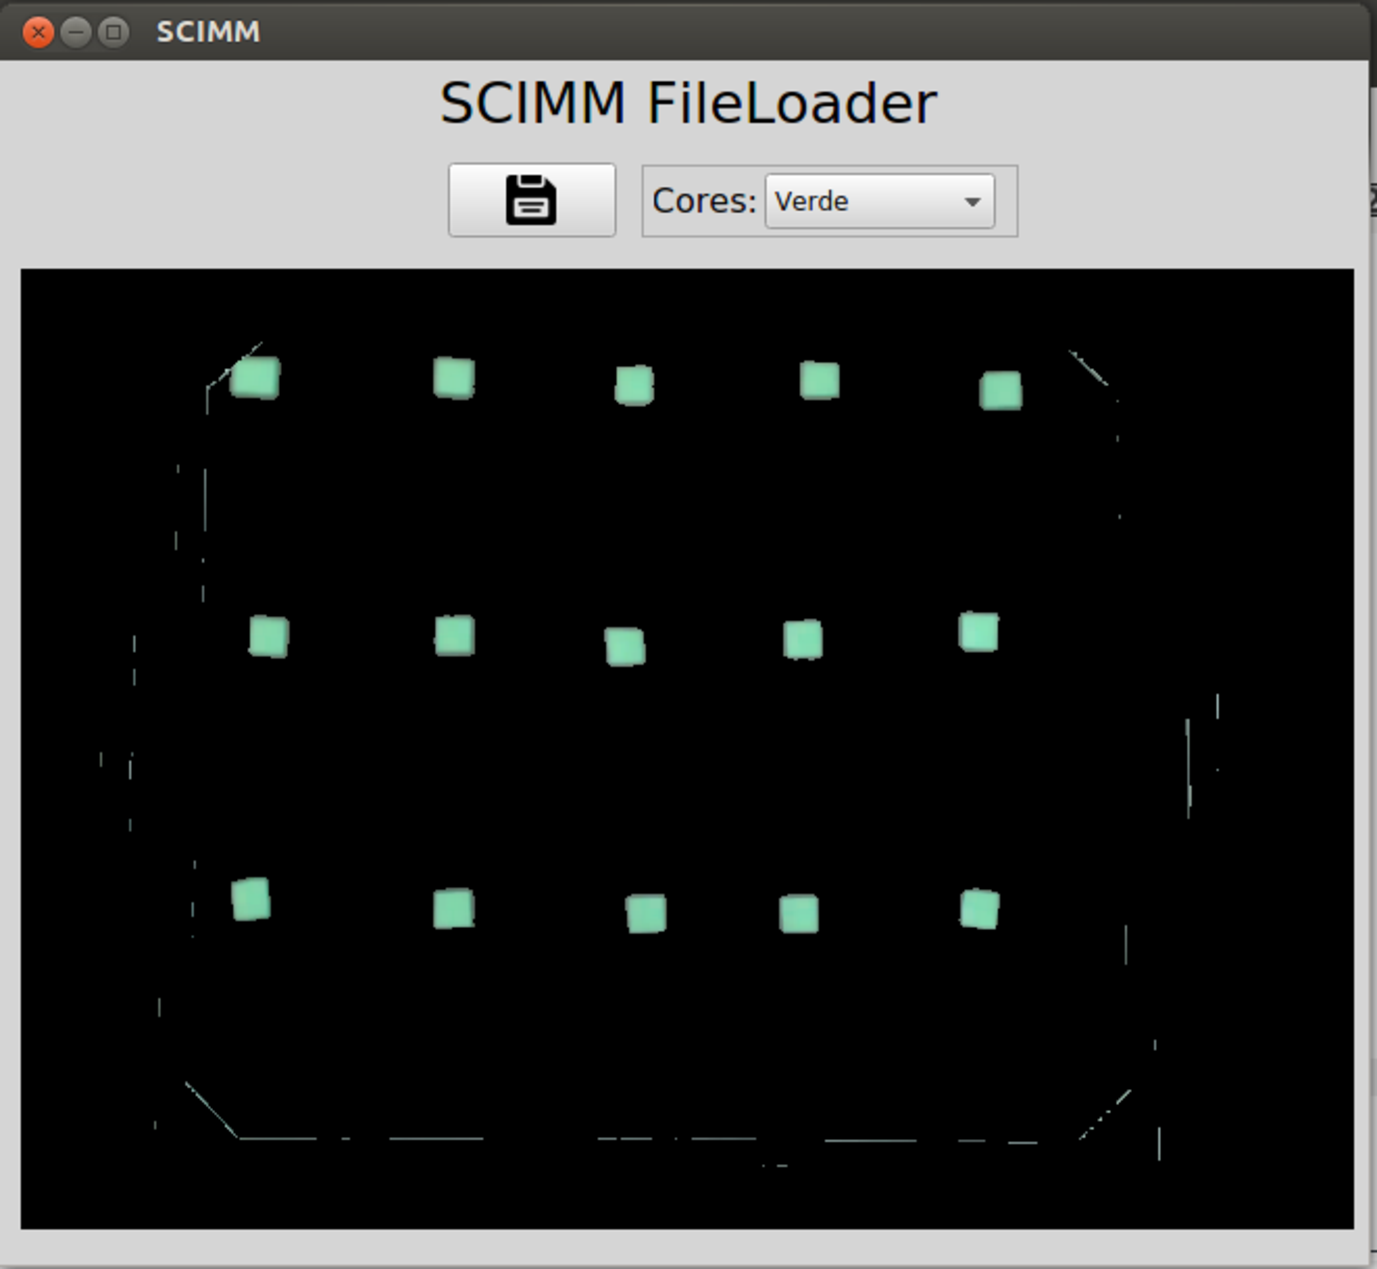
\includegraphics[width=\textwidth]{/testes/verde.pdf}
			\caption{Objetos da cor verde}
			\label{fig:verde}
		\end{minipage}
	\end{figure}

	O detalhamento das quantidades e porcentagens dos objetos encontrados está na Tabela \ref{tab:verde}.
\begin{table}[h]
\centering
\begin{tabular}{l|c|c}
Tipo de Objeto & Quantidade & \% \\ % Note a separação de col. e a quebra de linhas
\hline                               % para uma linha horizontal
Objetos Completos &  15 &100 \\
\hline 
Objetos Com Falha de Preenchimento & 0\\
\hline 
Objetos Com Diminuição de Contorno &  0\\
\hline 
Objetos Com Diminuição de Área &  0 \\
\hline 
Objetos Com Falhas Críticas & 0 \\
\hline \hline 
Objetos Extrapolados & 0 \\
\hline 
\end{tabular}
\caption{Categorização Dos Objetos}
\label{tab:verde}
\end{table}	
\newpage
\subsubsection{Rosa}

	
Dentre os objetos Rosa detectados, quatro obtiveram falhas críticas em sua detecção, devido ao mal preenchimento e a deformação/diminuição de contorno, partes A, B, D e M do campo.
	
	\begin{figure}[H]
		\begin{minipage}[b]{0.45\linewidth}
			\centering
			\includegraphics[width=\textwidth]{campodivisao.pdf}
			\caption{Divisão do campo.}				
		\end{minipage}
		\hspace{0.5cm}
		\begin{minipage}[b]{0.45\linewidth}
			\centering
			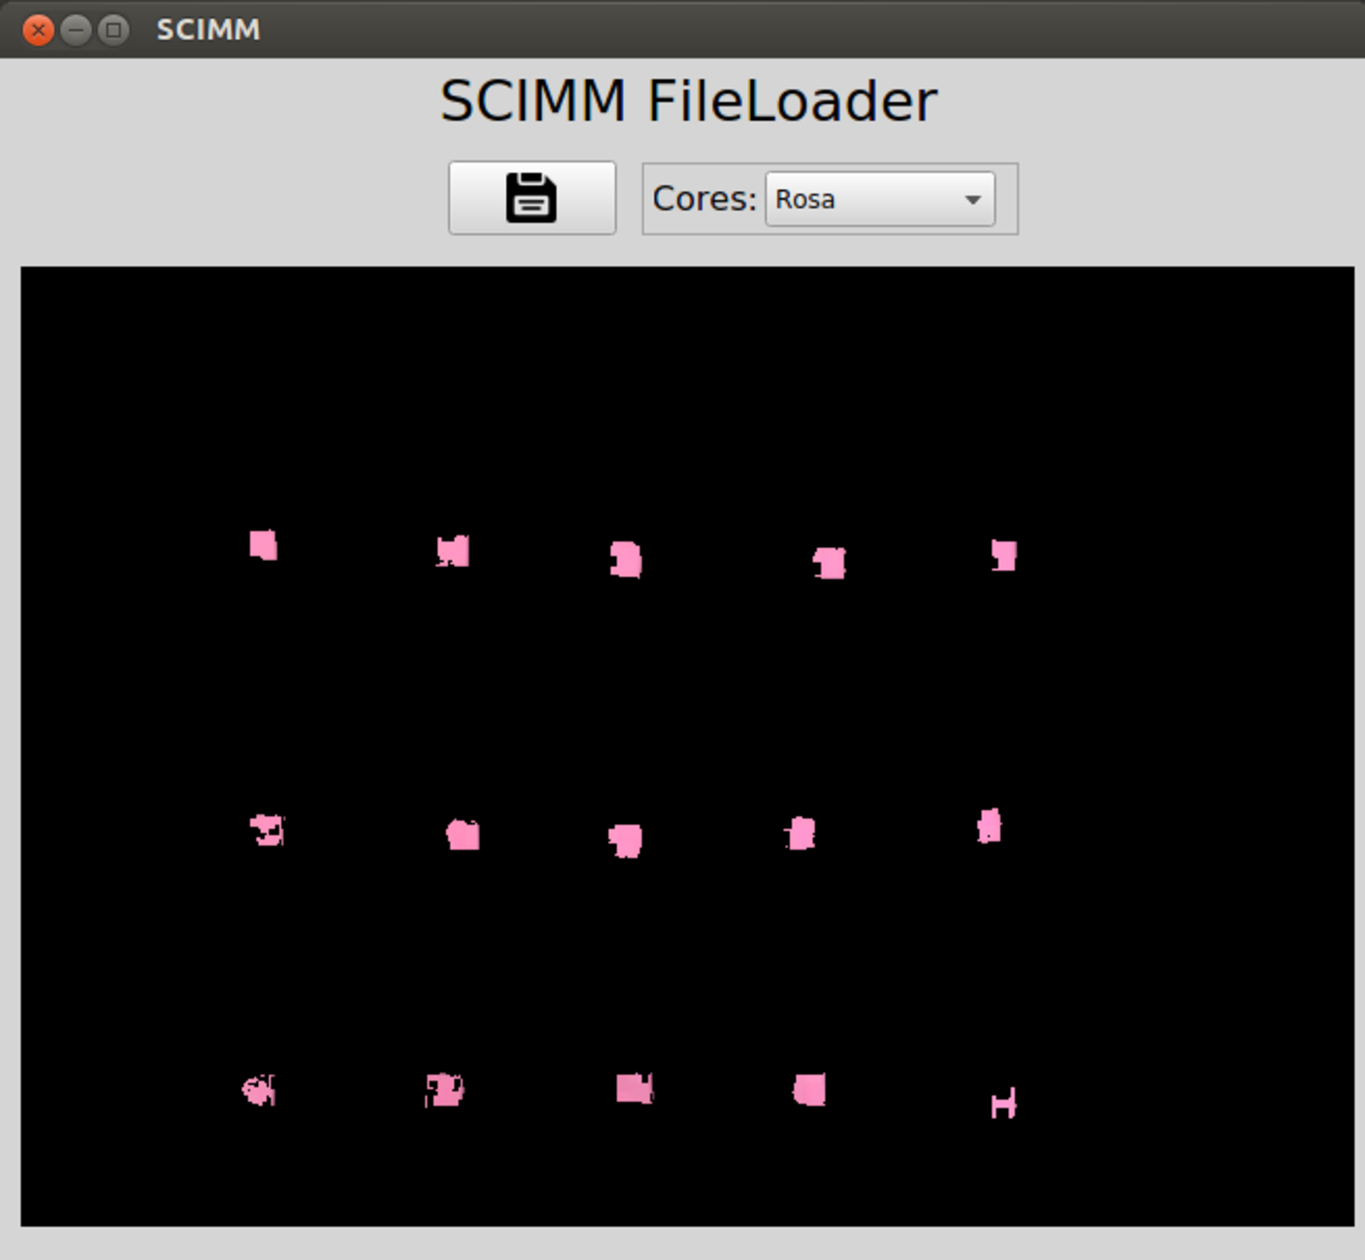
\includegraphics[width=\textwidth]{/testes/rosa.pdf}
			\caption{Objetos da cor rosa}
			\label{fig:rosa}
		\end{minipage}
	\end{figure}

 Dentre os onze restantes: três foram detectados com um pequena diminuição de área, partes K, N e O; os outros oito foram encontrados apenas com diminuição de contorno (Figura \ref{fig:rosa}).  O detalhamento das quantidades e porcentagens dos objetos encontrados está apresentado na Tabela \ref{tab:rosa},
	
	\begin{table}[H]
\centering
\begin{tabular}{l|c|c}
Tipo de Objeto & Quantidade  & \% \\ % Note a separação de col. e a quebra de linhas
\hline                               % para uma linha horizontal
Objetos Completos &  0\\
\hline 
Objetos Com Falha de Preenchimento & 0\\
\hline 
Objetos Com Diminuição de Contorno & 8& 53,33
 \\
\hline 
Objetos Com Diminuição de Área & 3 & 20\\
\hline 
Objetos Com Falhas Críticas & 4 & 26,66 \\
\hline \hline 
Objetos Extrapolados & 0 \\
\hline 
\end{tabular}
\caption{Categorização Dos Objetos}
\label{tab:rosa}
\end{table}

Dentre as classificações dos objetos as que descaracterizam o objeto para detecção são:  \textit{Objetos Com Falhas Críticas} e \textit{Objetos Com Falha de Preenchimento} que juntos somam 26,66\% dos objetos. Apesar de ser um erro bastante significativo, não é de costume da equipe Cedro utilizar a cor rosa como marcadores de robôs em seus jogos, sendo assim, essa taxa de erro não influenciará na eficiência do sistema.
\newpage
\subsubsection{Roxo}


Todos os objetos roxos dispostos no campo foram encontrados pelo intervalo da cor(Figura \ref{fig:roxo}).

\begin{figure}[H]
	\begin{minipage}[b]{0.45\linewidth}
		\centering
		\includegraphics[width=\textwidth]{campodivisao.pdf}
		\caption{Divisão do campo.}				
	\end{minipage}
	\hspace{0.5cm}
	\begin{minipage}[b]{0.45\linewidth}
		\centering
		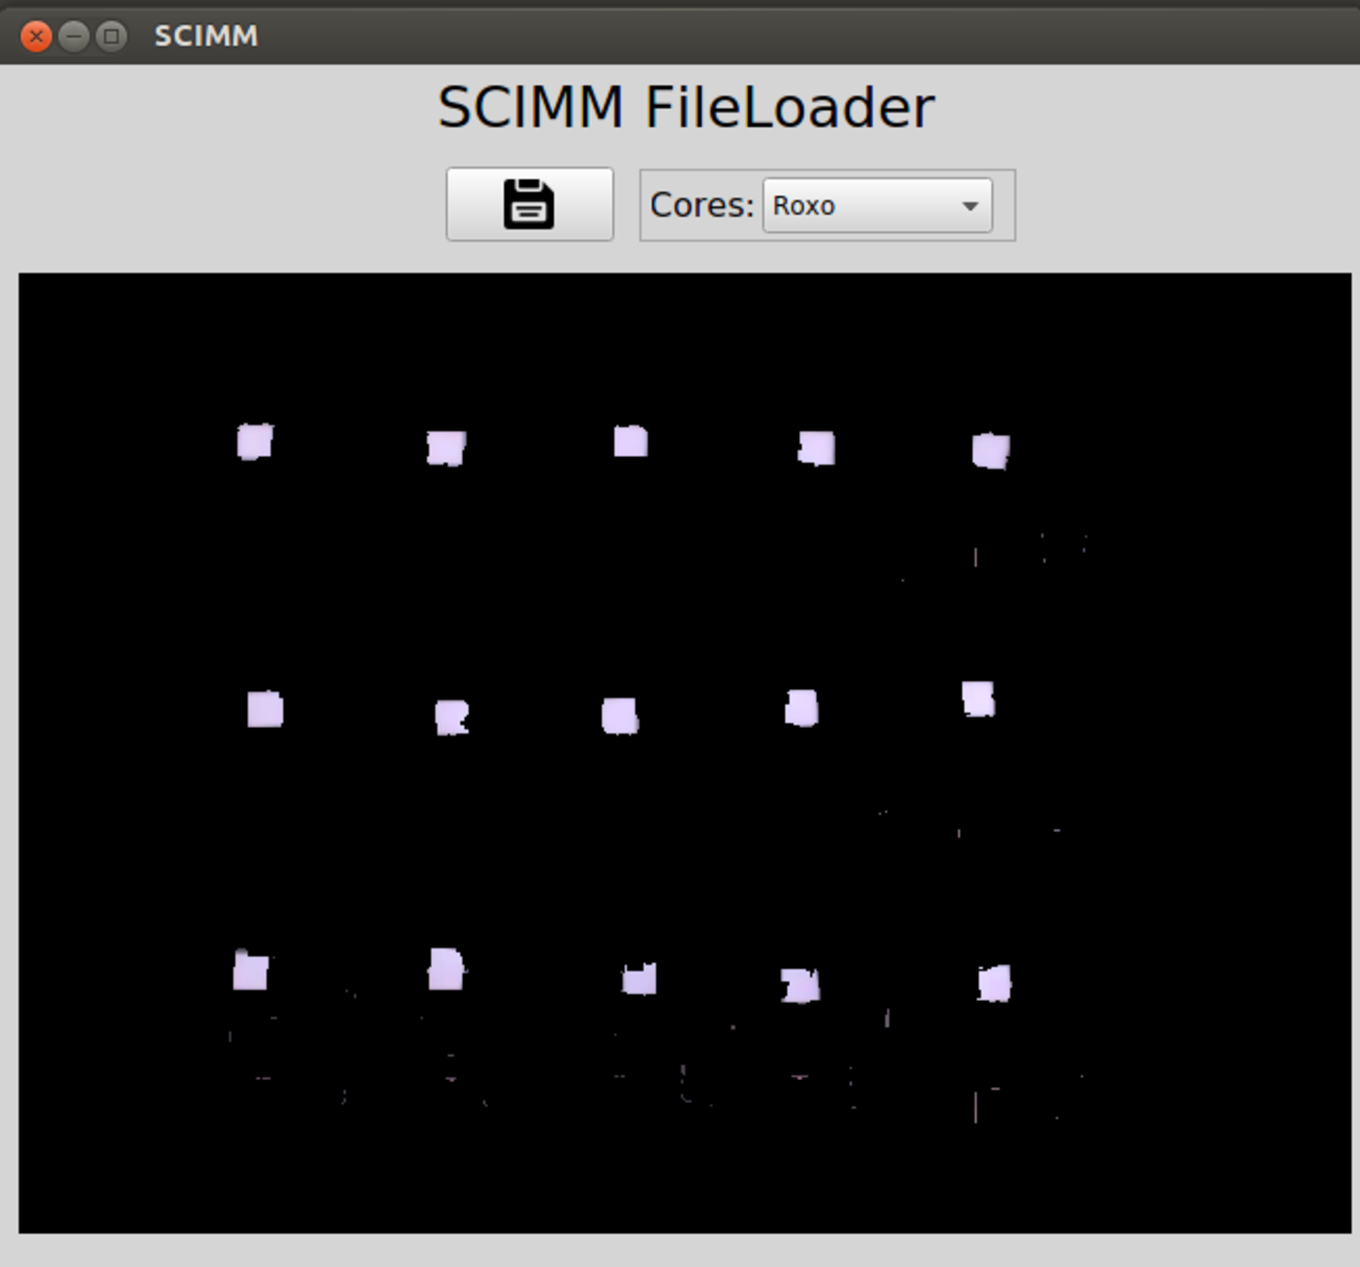
\includegraphics[width=\textwidth]{/testes/roxo.pdf}
		\caption{Objetos da cor roxo}
		\label{fig:roxo}
	\end{minipage}
\end{figure}

 Dentre os quinze, quatro não apresentaram problema algum e foram completamente detectados, partes B, I, H e N do campo; três apresentaram diminuição de área, partes E, G e J, e oito possuíram diminuição em seu contorno. O detalhamento das quantidades e porcentagens dos objetos encontrados está na Tabela \ref{tab:roxo}.
\begin{table}[H]
\centering
\begin{tabular}{l|c|c}
Tipo de Objeto & Quantidade  & \% \\ % Note a separação de col. e a quebra de linhas
\hline                               % para uma linha horizontal
Objetos Completos &  4 & 26,66\\
\hline 
Objetos Com Falha de Preenchimento & 0 \\
\hline 
Objetos Com Diminuição de Contorno &  8 & 53,33\\
\hline 
Objetos Com Diminuição de Área & 3 & 20\\
\hline 
Objetos Com Falhas Críticas & 0 \\
\hline \hline 
Objetos Extrapolados & 0 \\
\hline 
\end{tabular}
\caption{Categorização Dos Objetos}
\label{tab:roxo}
\end{table}
	\newpage
\subsection{Cores Com Problemas}
Cores como Vermelho e Laranja possuem o problema de por vezes, devido a interferência externa, se assemelharem a outras. Este problema é observado por todas as equipes participantes das competições do VSSS.
	
\subsubsection{Vermelho}


A cor rosa, em determinadas luminosidades pode acabar sendo semelhante a cor vermelha, por este motivo, alguns traços dos objetos rosas estão aparecendo dentro do intervalo de calibração(Figura \ref{fig:vermelho}), mas não configuram um objeto.
		\begin{figure}[H]
			\begin{minipage}[b]{0.45\linewidth}
				\centering
				\includegraphics[width=\textwidth]{campodivisao.pdf}
				\caption{Divisão do campo.}				
			\end{minipage}
			\hspace{0.5cm}
			\begin{minipage}[b]{0.45\linewidth}
				\centering
				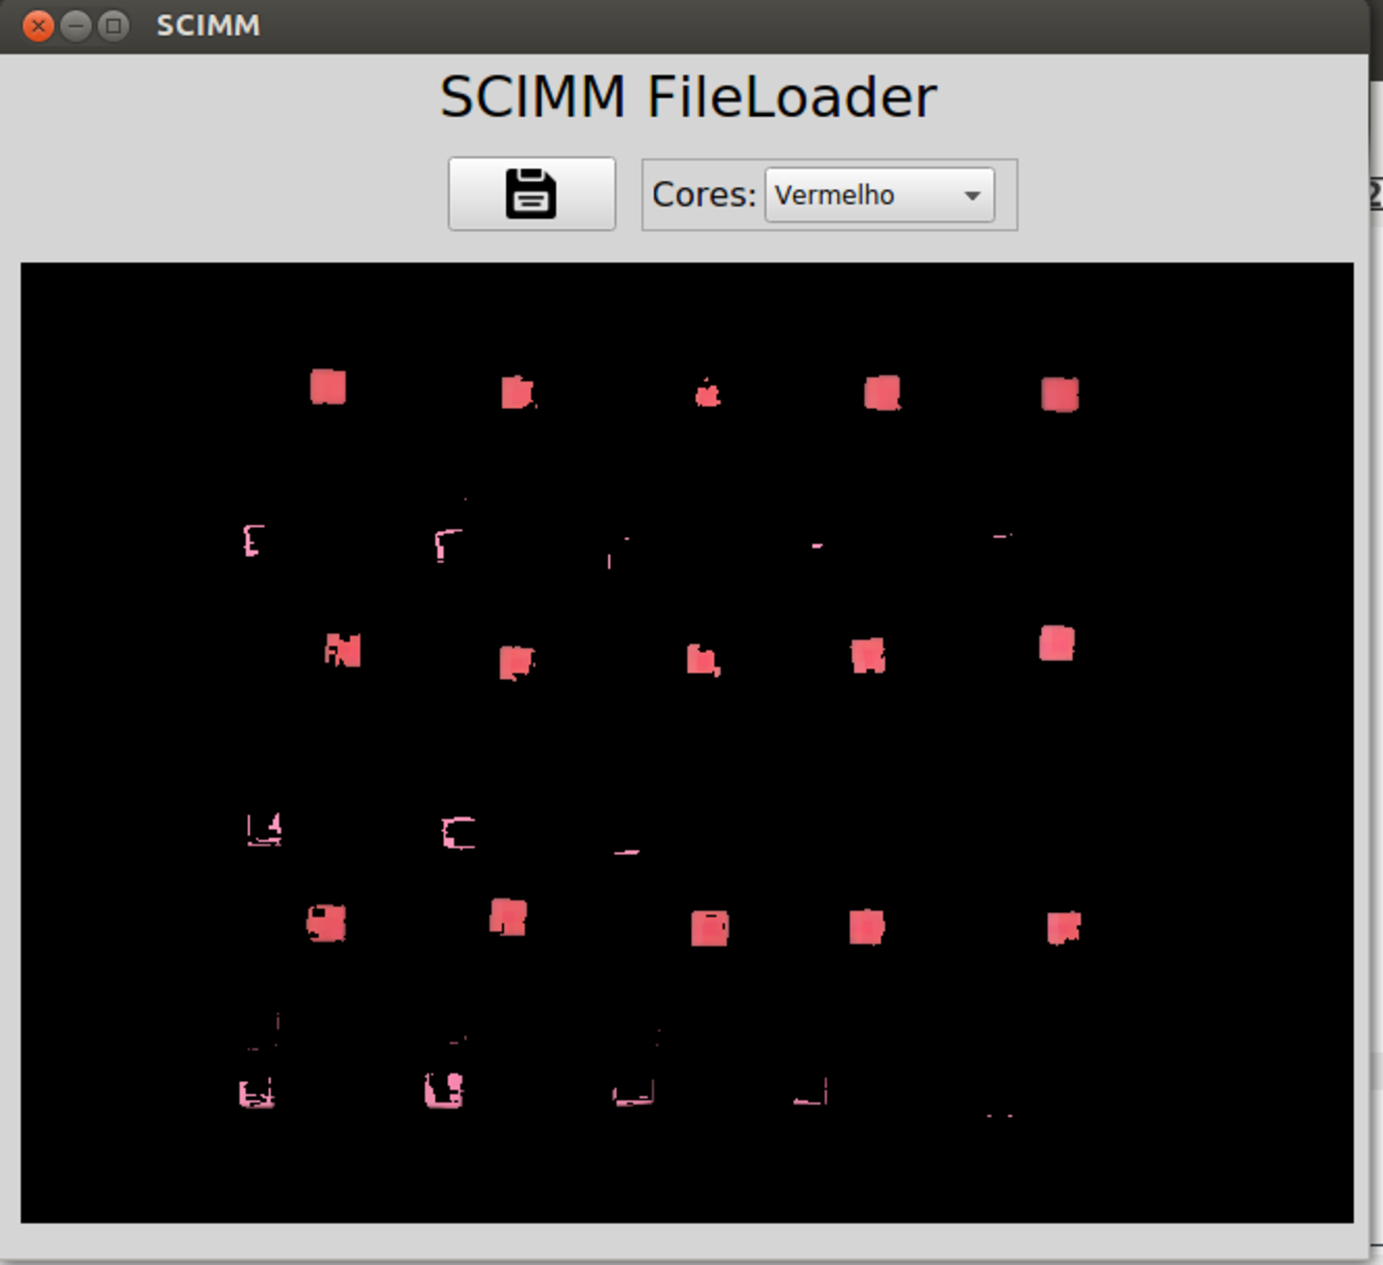
\includegraphics[width=\textwidth]{/testes/vermelho.pdf}
				\caption{Imagem somente com os objetos dentro do intervalo do valor da cor vermelho}
				\label{fig:vermelho}
			\end{minipage}
		\end{figure}
		
		
Dos 15 marcadores da cor vermelha, 2 apresentaram falha de preenchimento, parte A e B do campo; 4 apresentaram diminuição de contorno, presentes nas partes E, F, H e M; 1 apresentando falha crítica, parte I do campo, e 8 foram encontrados de forma completa.  
Dentre as classificações, as que 
descaracterizam o objeto para detecção são: \textit{Objetos Com Falhas Críticas} e \textit{Objetos Com Falha de Preenchimento} que juntos somam somente 19,99\% dos objetos. As quantidades e porcentagens dos demais objetos podem ser vistas na Tabela~\ref{tab:vermelho}.
	
	\begin{table}[H]
\centering
\begin{tabular}{l|c|c}
Tipo de Objeto & Quantidade  & \% \\ % Note a separação de col. e a quebra de linhas
\hline                               % para uma linha horizontal
Objetos Completos &  8 & 53,33 \\
\hline 
Objetos Com Falha de Preenchimento & 2 & 13,33 \\
\hline 
Objetos Com Diminuição de Contorno &  4 & 26,66 \\
\hline 
Objetos Com Diminuição de Área &  0  & 0 \\
\hline 
Objetos Com Falhas Críticas &  1 & 6,66\\
\hline \hline 
Objetos Extrapolados &  13 \\
\hline 
\end{tabular}
\caption{Categorização Dos Objetos}
\label{tab:vermelho}
\end{table}



\subsubsection{Laranja}

	
	Devido a um problema muito comum na área de calibração de cores, a cor laranja possui a característica de ser, por muitas vezes, semelhante a vermelha(Figura \ref{fig:laranja}). Devido ao fator luminosidade, tanto laranja quanto vermelho, tendem a se tornarem próximas.
		
		\begin{figure}[H]
			\begin{minipage}[b]{0.45\linewidth}
				\centering
				\includegraphics[width=\textwidth]{campodivisao.pdf}
				\caption{Divisão do campo.}				
			\end{minipage}
			\hspace{0.5cm}
			\begin{minipage}[b]{0.45\linewidth}
				\centering
				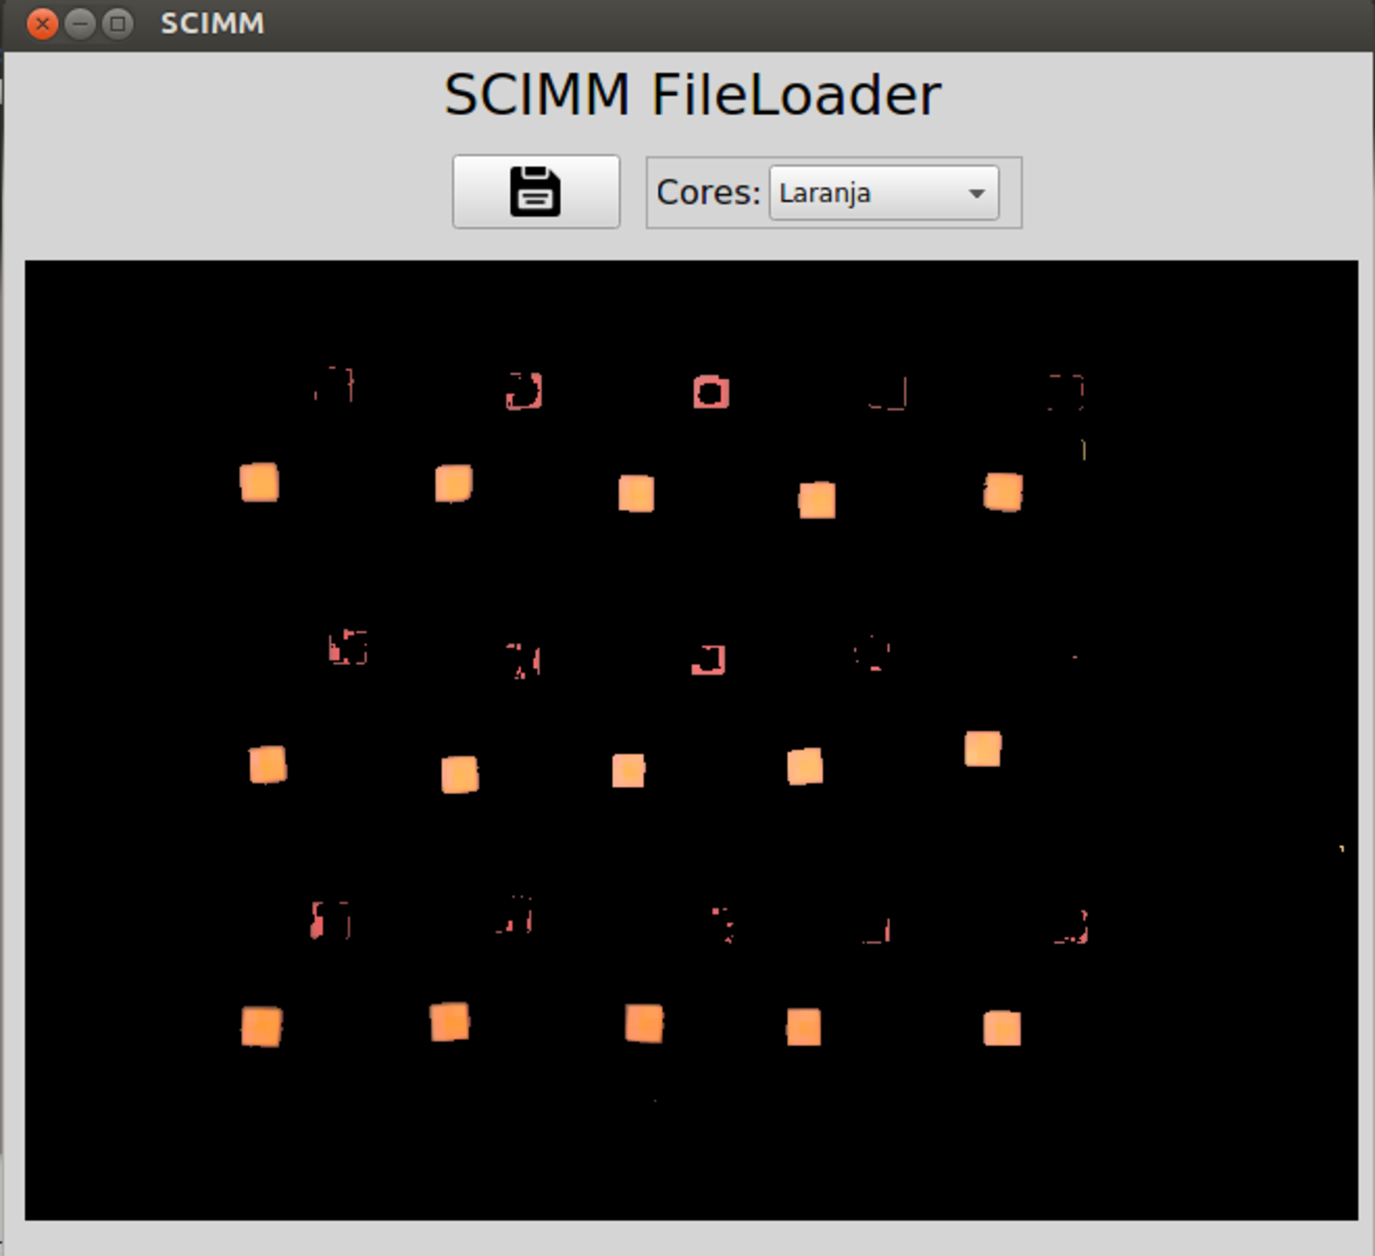
\includegraphics[width=\textwidth]{/testes/laranja.pdf}
				\caption{Objetos da cor laranja}
				\label{fig:laranja}
			\end{minipage}
		\end{figure}
	Sabendo deste problema, o fato de terem sido encontrados objetos da cor vermelha dentro do intervalo de valores da cor laranja é ignorado, e somente serão levados em consideração os objetos visualmente laranjas.
	Os quinze objetos da cor laranja foram encontrados com precisão. Todos possuindo seu completo preenchimento e borda. As quantidade e porcentagens do objetos estão disposto na Tabela \ref{tab:laranja}.
	
\begin{table}[H]
\centering
\begin{tabular}{l|c|c}
Tipo de Objeto & Quantidade  & \% \\ % Note a separação de col. e a quebra de linhas
\hline                               % para uma linha horizontal
Objetos Completos &  15 & 100 \\
\hline 
Objetos Com Falha de Preenchimento & 0 \\
\hline 
Objetos Com Diminuição de Contorno &  0 \\
\hline 
Objetos Com Diminuição de Área &  0 \\
\hline 
Objetos Com Falhas Críticas & 0 \\
\hline \hline 
Objetos Extrapolados & 8 \\
\hline 
\end{tabular}
\caption{Categorização Dos Objetos}
\label{tab:laranja}
\end{table}
\newpage
\subsection{Análise Geral}
Estavam disposto pelo campo 105 objetos coloridos, sendo a maioria detectado perfeitamente e alguns com falhas. Na Figura \ref{fig:total}, pode ser observada a quantidade de objetos que se encontram em cada uma das categorias. Destes, 66,7\% dos objetos foram encontrados corretamente, 1,9\% foram encontrados com falhas de preenchimento, 20\% apresentaram perda de contorno, 6,67\% apresentaram diminuição da área e 4,76\% apresentaram falhas e faltas que prejudicaram totalmente o objeto.
	\begin{figure}[H]
		\centering
		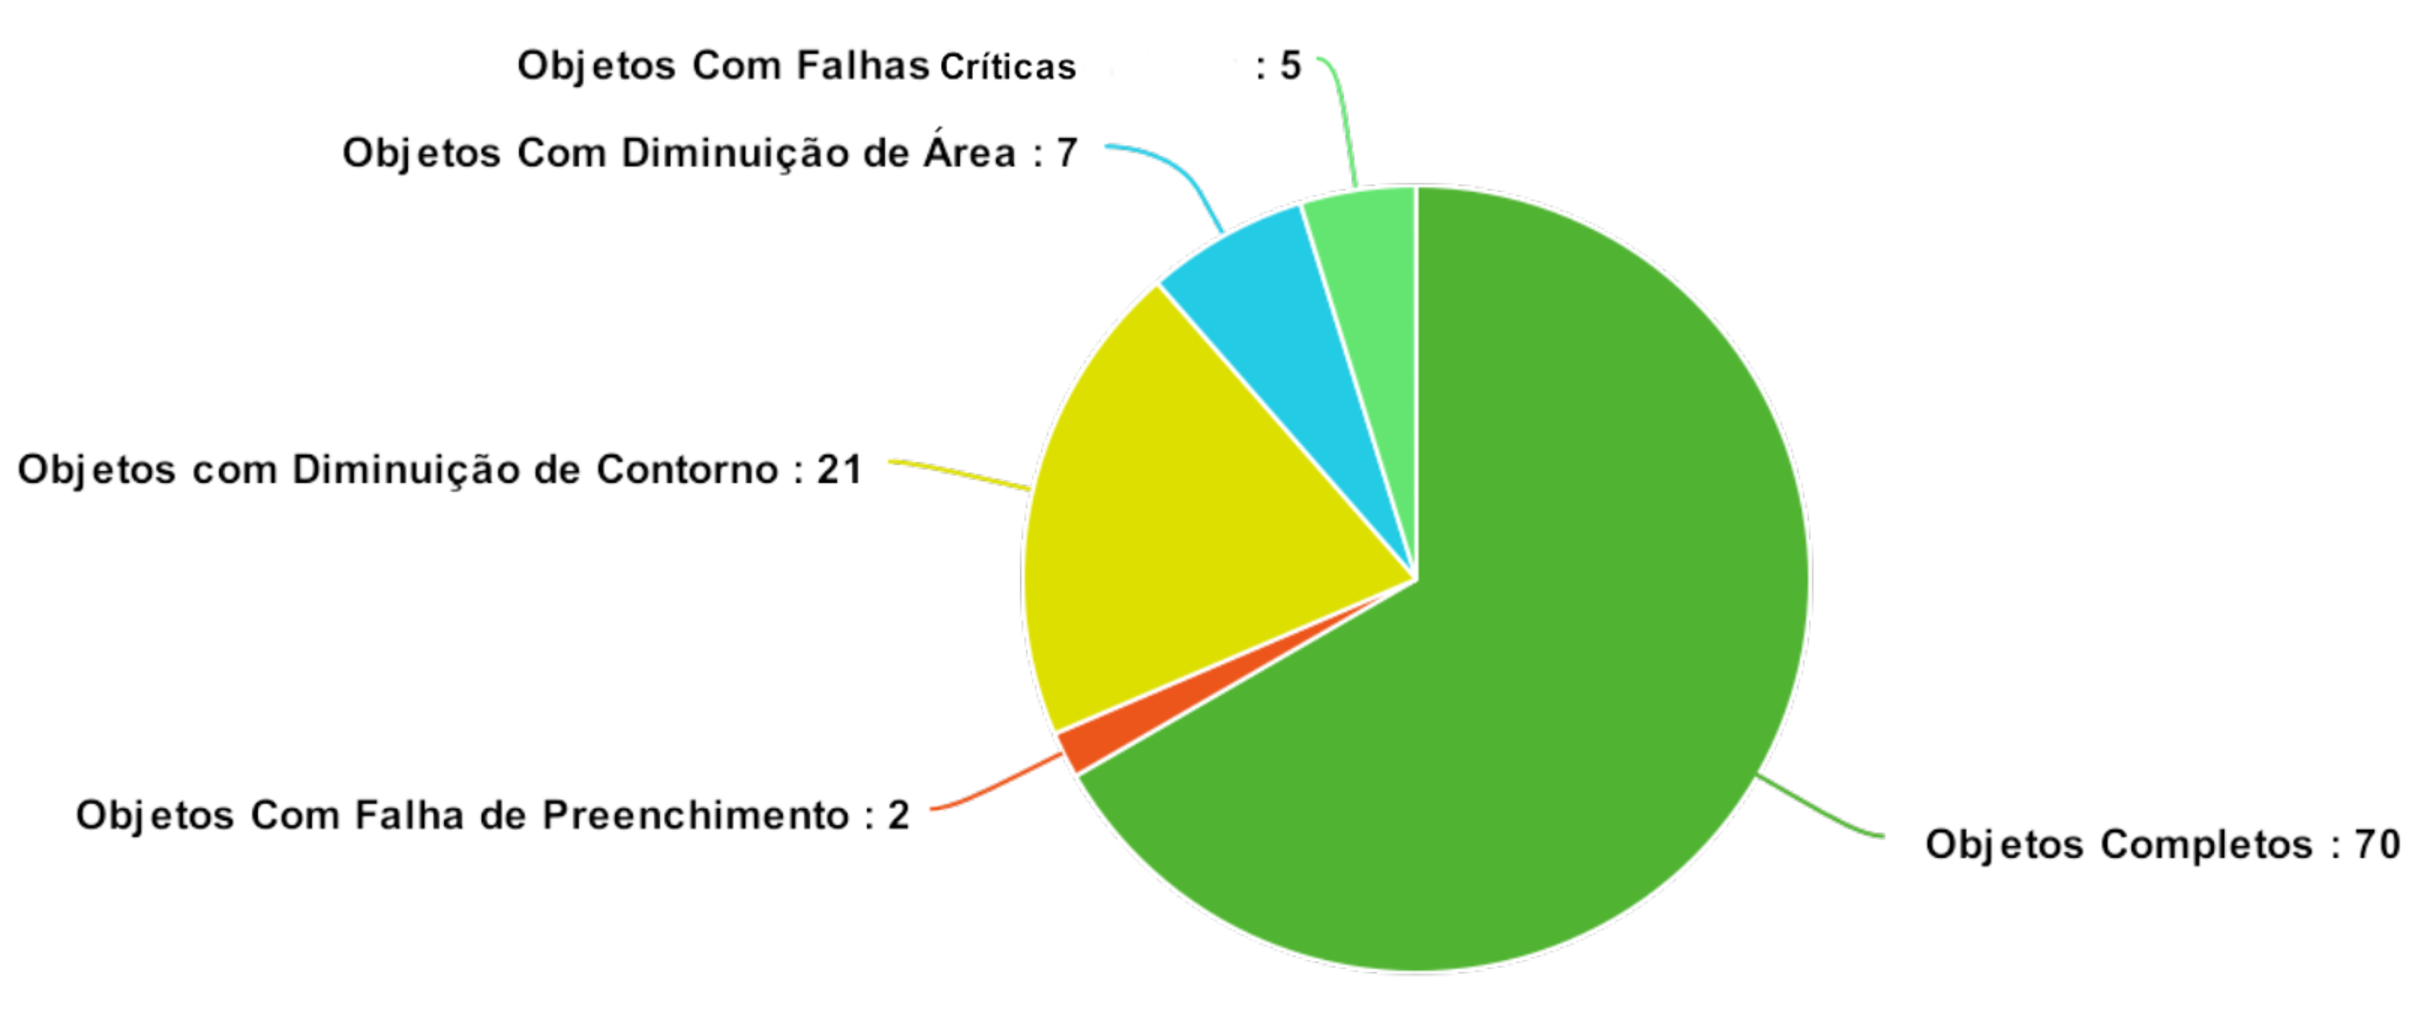
\includegraphics[width=0.8\textwidth]{/testes/graficotestes.pdf}
		\caption{Gráfico de análise do resultado dos testes}
		\label{fig:total}
	\end{figure}
	
	
	Analisando-se estes valores, pode-se perceber que os erros considerados críticos na detecção de objetos por meio da sua cor são \textit{Objetos Com Falhas Críticas} e \textit{Objetos Com Falha de Preenchimento} que juntos somam 6,67\% dos objetos.
	
	\section{Considerações Finais}
	
	Pode-se concluir que o sistema SCIMM, atingiu seus objetivos de calibração automática das cores para utilização no Futebol de Robôs categoria VSSS, pois apresentou ótimos resultado com as cores amarelo, azul, laranja e verde, resultados bons com a cor vermelha, e resultados satisfatório com a cor roxo. Resultados pouco satisfatórios foram obtidos utilizando-se a cor rosa. 
	
	As cores calibradas pelo sistema, quando testadas em ambiente de detecção de objetos coloridos, simbolizaram 98 dos 105 objetos, conseguindo com que somente 7 objetos coloridos não tenham sido identificados.
	
	A automatização do processo de calibração levou em média 5 minutos, 1/4 do tempo disponível para ajustes do time durante as competições.